\section{Attack Analysis}
The flow of credential information in the overall system currently originates within a web browser context. This is then parsed through a virtual serial channel to the auxiliary MCU where the information is encrypted and stored on the EEPROM based filesystem. A series of experiments were constructed to test the confidentiality, integrity and availability of data within the overall system. It is important to ensure that each endpoint of the system is thoroughly tested and secured to meet these key security objectives. Three experiments will be conducted in this section to quantify the level at which these key security objectives have been met.


\subsection{Experiment 1 - Malware and Serial Tap}

Various attack vectors exist which are aimed at compromising sensitive data such as credentials. Two methods of credential extraction will be attempted, the first involves a malicious modification to the browser extension and the second involves tapping into the serial communications between the auxiliary MCU and USB driver MCU.

With regards to the first method of credential extraction, most browsers implement a policy known as CORS (Cross-Origin Resource Sharing) which prevents JavaScript code on one website from making HTTP requests to another non related website. However a communications technology known as WebSockets exists and it is not bound by CORS which makes it ideal for password extraction.

\subsubsection{Requirements}

\begin{itemize}
  \item A web server
  \item SSL certificate 
  \item WebSocket server 
  \item WebSocket client 
  \item CP2102 (USB to serial board) 
  \item End Device 
\end{itemize}


Due to the restrictions imposed on modern browsers, it is no longer possible to host SSL based secure WebSocket servers (WSS) using self signed certificates, doing so will raise the \textbf{ERR\_CERT\_AUTHORITY\_INVALID} error message in google chrome. Rather WebSocket servers must run on a dedicated host who has obtained an SSL certificate from a legitimate certificate authority. For the purposes of this experiment the web host at \textbf{www.lunar.sh} was made available to the author which had obtained an SSL certificate from certbot, a python based SSL certificate manager from Let's Encrypt. With this the WebSocket server was written in Python using the \textbf{WebSockets} library. This may be installed with the following command:

\begin{lstlisting}[language=bash, frame=none]
$ sudo pip3 install WebSockets
\end{lstlisting}

The source code for the WebSocket sever is shown in \hyperref[sec:exp1]{Appendix E.1}.

The relevant certificate and private key PEMs were imported and the WebSocket server binded to port 4444. Next a DNS entry (A Record) for \textbf{cmd.lunar.sh} was created and the WebSocket client written in JavaScript. The following line of code was inserted at the top of \textbf{background.js} (extension script):

\begin{lstlisting}[language=java]
let wss = new WebSocket('wss://cmd.lunar.sh:4444');
\end{lstlisting}

This would connect and establish a WebSocket connection to the host. The remaining task was to insert the following line of code at the appropriate location (in the onConnect port handler where a call to \textbf{native.postMessage} is made to encrypt the plaintext password) :
\begin{lstlisting}[language=java]
// line 100
// msg[1] contains the unencrypted password
wss.send("password: " + msg[1]);
\end{lstlisting}

For the second method of credential compromise Figure 7.1 shows the connections that need to be made to the USB driver MCU's serial port. It can be seen that the TX line of the driver MCU is connected to the RX line of the CP2102 and the RX line of the USB driver MCU should be connected to the connected to the TX line of the CP2102.
\begin{figure}[H]
\centering
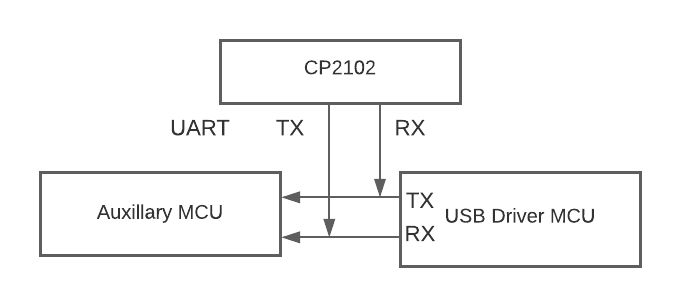
\includegraphics[width=0.6\columnwidth]{Figures/Fig_49.png}
\caption{SP2102 connection to host device.}
\label{fig:gantt}
\end{figure}

\subsubsection{Method}
Once all the requirements were in place the procedure for the experiment then consisted of visiting a website login portal (outlook was used in this case) , entering a username (test\_user) and password (testing123\#) and selecting the 'Store Credential' button in the extension UI (Figure 5.3). This would trigger the exploit and transmit the password to the remote endpoint controlled by an attacker. The exchange of serial data would also be captured by the CP2102 board during encryption. 

The time taken to perform both methods of password compromise was captured for three different password encryption stages using a software timer (\hyperref[sec:timerp]{Appendix E.4}).
\subsubsection{Results}
Figure 7.2 depicts the results of the first method of credential extraction. The results were captured during an SSH session with the remote web server. It is seen to consist of the IP address of the remote client as well as the plain-text password the user had entered when requesting that the browser extension save the credential information to EEPROM storage. 

\begin{figure}[H]
\centering
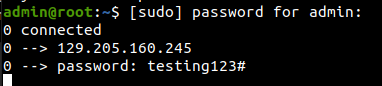
\includegraphics[width=0.6\columnwidth]{Figures/Fig_28.png}
\caption{WebSocket server results.}
\label{fig:gantt}
\end{figure}

The Arduino serial monitor was used to monitor the incoming data delivered to the CP2102 board. After the 'Store Credential' button was clicked the following serial text data was captured:

\begin{lstlisting}[language=bash, frame=none]
$encrypt$ADE2...$test_user|!#|testing123#$R01$
\end{lstlisting}

The measured credential acquisition times are shown in Table 10. It can be seen that method 2 (using the CP2102 board) was the fastest at capturing passwords with an average acquisition time of 60.2 ms. This was then followed by method 1 with an average time of around 552 ms.

It should be noted that the acquisition times for method 1 is highly dependant on the bandwidth of the client-server web-socket connection.

\begin{table}[H]
\centering
\begin{tabular}{lllll}
Method & t1 /ms & t2 /ms & t3 /ms & avg /ms \\
1      & 552.0   & 550.0  & 555.0  & 552.3    \\
2      & 60.5    & 57.5   & 62.5   & 60.2     
\end{tabular}
\caption{Time to acquire data with each method.}
\end{table}

The results show that it is possible for an attacker to relay information from a malicious browser extension to a remote server. Additionally by tapping into the serial connection of the USB driver MCU it was shown that an attacker could extract the credential plain-text.

The flow of credential information during password storage is shown in Figure 7.3. Data leakage involves intercepting either the key modulus or password either through monitoring of the serial communications communications channels or malware (demonstrated through WebSocket interception).

Preventing third party monitoring of sensitive information may involve encrypting the serial communications channel itself from end to end so that an attacker cannot decipher information so easily. 
\begin{figure}[H]
\centering
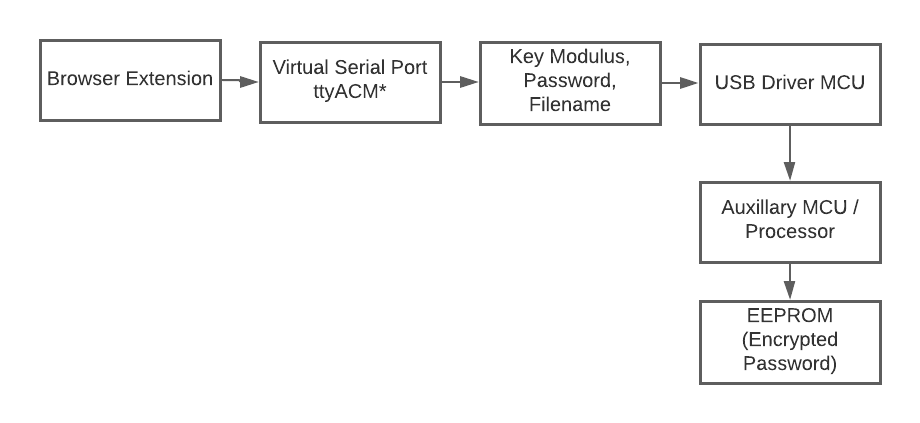
\includegraphics[width=0.8\columnwidth]{Figures/Fig_30.png}
\caption{Flow of data during password storage/encryption.}
\label{fig:gantt}
\end{figure}

A data confidentiality matrix was created and is shown in Table 11. For each acquisition method the requirement as well as risk is highlighted. For example in method 1 browser malware was created, due to the ease with which a malicious extension can be installed this was labeled as a high risk. Method 2 involved tapping the serial connection of the USB driver MCU, this requires physical access to the device and so was labeled as low risk.

Finally two additional types of acquisition method were included, the first is decryption through master key leakage, this requires an attack to have remote access to the host operating system and was labeled as medium risk. Finally code injection follows and requires an injector to function and was again labeled as medium risk.
\begin{table}[H]
\centering
\begin{tabular}{|l|l|l|}
\hline
Method              & Requires        & Risk   \\ \hline
1 (Browser Malware) & Software Access & High   \\ \hline
2 (Serial Tap)      & Physical Access & Low    \\ \hline
Master Key          & Remote Access   & Medium \\ \hline
Code Injection      & Software Access & Medium \\ \hline
\end{tabular}
\caption{Data confidentiality risk matrix.}
\end{table}

\subsection{Experiment 2 - Denial of Service}
Denying legitimate users the ability to use services on the end system is also a real possibility which must be protected against. Currently three bottlenecks exist in the overall system. These are the processing time required to encrypt passwords and the filesystem formatting time, which are both on the order of a few seconds. The third bottleneck is then the throughput of the serial connection which is around 115200 bps.

Due to the fact that communication is over a serial connection, a major flaw automatically exists, which is that a serial connection/stream can be locked using the TIOCEXCL TTY ioctl in Linux to prevent other file open/connection attempts from succeeding. This means that an attacker only has to craft an application that opens a serial connection, sets the relevant ioctl and sits idle to perform a DoS attack, preventing the native host from establishing a connection to the USB host MCU.

Finding bugs in the source code for the auxiliary MCU could also lead to the discovery of potential DoS vectors. Upon testing the various inputs and outputs of the supported serial commands a bug was found in the command processor for the auxiliary MCU. If a large number of command requests per second with malformed parameters was submitted over the serial channel the auxiliary MCU would lock up due to memory exhaustion/buffer overflows.

Additionally the insertion of serial commands (i.e to format and encrypt at random) is also another vector that could be employed by an attacker to render services unavailable.

\subsubsection{Requirements}

\begin{itemize}
  \item C++ DoS client
  \item Software client
  \item Host device
\end{itemize}

The C++ DoS client utilizes the \textbf{serialib} library to perform command flooding over the serial port. The source code of the DoS client is shown in \hyperref[sec:exp2]{Appendix E.2}.

\subsubsection{Method}
The procedure for the experiment consisted of connecting the host device to a computer and then launching the DoS client. One of the two DoS methods would then be selected and executed. After successful execution of a DoS exploit a google chrome browser instance would be launched and operations performed on the browser extension including decrypting user passwords and storing passwords. Additionally an instance of the Arduino serial monitor was launched to determine if command interaction with the host device was possible following a DoS exploit.

Finally the time taken to reach an unusable state using both methods was recorded using a software timer (\hyperref[sec:timerc]{Appendix E.5}) for three iterations of encryption.

\subsubsection{Results}

Figure 7.5 shows the error message obtained from the Arduino serial monitor as a result of the first method of DoS attack (TIOCEXCL lock). As can be seen no serial port access was possible and the google chrome browser extension became unresponsive following the exploit. These results show that it is possible for an attacker to craft a malicious application that interferes with the legitimate operation of the software client.

\begin{figure}[H]
\centering
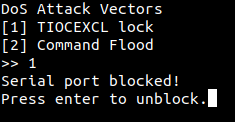
\includegraphics[width=0.35\columnwidth]{Figures/Fig_32.png}
\caption{DoS client prompt. Option 1 execution.}
\label{fig:gantt}
\end{figure}

Figure 7.4 depicts the user interface of the DoS client. It is seen to consist of a menu with two options available (corresponding to the two DoS attack vectors).
\begin{figure}[H]
\centering
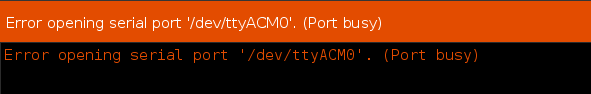
\includegraphics[width=0.9\columnwidth]{Figures/Fig_31.png}
\caption{Arduino serial monitor error.}
\label{fig:gantt}
\end{figure}

Figure 7.6 shows the prompt displayed when the second DoS attack vector was selected (Command Flood). Figure 7.7 showcases the browser extension's unresponsiveness following the DoS attack. As can be seen the loading indicator was continuously active and it was not possible to store or decrypt passwords. Only a hard reset (through switching the host device's power supply on and off) and a restart of google chrome fixed the issues encountered.  
\begin{figure}[H]
\centering
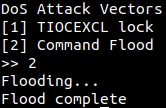
\includegraphics[width=0.25\columnwidth]{Figures/Fig_33.png}
\caption{DoS client prompt. Option 2 execution.}
\label{fig:gantt}
\end{figure}


\begin{figure}[H]
\centering
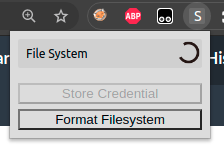
\includegraphics[width=0.3\columnwidth]{Figures/Fig_88.png}
\caption{Browser extension. Unresponsive after command flood.}
\label{fig:gantt}
\end{figure}

For command flooding, it was found that by adjusting the variable \textbf{count\_max} different outage times (time taken to become responsible) could be realised. Table 12 shows the resulting outage times for a range of count\_max from 0 to 6000.
\begin{table}[H]
\centering
\begin{tabular}{llllllll}
count\_max     & 0         & 1000 & 2000 & 3000 & 4000 & 5000 & 6000 \\
outage time 1 /s & +infinity & 6.5  & 3.2  & 1.7  & 0.7  & 0.6  & 0.6 \\
outage time 2 /s & +infinity & 6.4  & 3.3  & 1.5  & 0.8  & 0.4  & 0.5 \\
outage time 3 /s & +infinity & 6.9  & 3.5  & 1.6  & 0.9  & 0.5  & 0.5\\
average time /s & +infinity & 6.6  & 3.3  & 1.6  & 0.8  & 0.5  & 0.5
\end{tabular}
\caption{Outage times for different count\_max}
\end{table}

Figure 7.8 is a graphical representation of Table 12. Initially for smaller values of count\_max it takes several seconds until a service outage occurs. Then gradually as count\_max is increased the time is seen to decrease exponentially until it reaches an asymptote around 0.5s. These results indicate that a large number of commands sent sequentially is enough to overwhelm the host device and that the minimum time needed for this to occur is around 0.5 seconds.
\begin{figure}[]
\centering
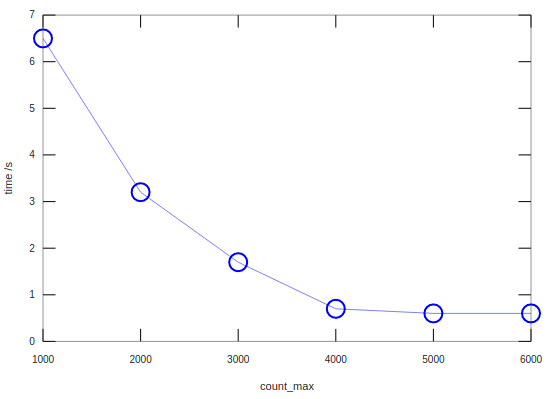
\includegraphics[width=0.75\columnwidth]{Figures/Fig_50.png}
\caption{count\_max vs time plot.}
\label{fig:gantt}
\end{figure}

Various countermeasures to the DoS vectors employed exist. A solution to the first vector employed is simply to lock the serial connection within the native client itself. It is only possible to lock a serial connection once and currently the native host does not lock its serial connection to the relevant ttyACM device. A solution to the second vector (Command Flood) is to introduce sleep functionality in the auxiliary MCU as well as serial buffer length checks in order to avoid buffer overflows. Better memory management should also feature in the auxiliary MCU to prevent memory exhaustion. 

All DoS vectors employed rely on running software on a computing device owned by the end user. In other words the security of the computing device running the software client is important to prevent DoS attacks. With respect to the host device itself, no major weaknesses were found when evaluating the ability to ensure availability of data. Therefore this key security objective was met in the final design.

\subsection{Experiment 3 - Code Injection}

The middle man native host, which is responsible for processing commands sent from the browser extension, is vulnerable to a range of code injection attacks aimed at capturing sensitive information traversing the communication pathway. Data such as the plain-text password and key modulus is sent over standard input and output to the native host where the JSON data is processed and the corresponding serial commands formatted and submitted the the USB driver MCU. The auxiliary MCU then performs the final command processing and results are then sent back to the native host over the serial channel where they can be relayed to the browser extension.

Code injection and method detouring relies on copying executable code to a target executable's memory image. Specifically the first few instruction bytes of a target function (\textbf{exec\_encrypt} in the case of the native host) is replaced with a jump to an alternative function (detour function) with the same formal parameters as the original. Custom behaviour, like writing the data to a file can then be implemented in the detour function. Furthermore the arguments to the original function could be modified in some unintended way, such as saving all passwords under a common phrase that an attacker controls. This experiment is designed to test the data integrity and confidentiality of the overall system.

\subsubsection{Requirements}

\begin{itemize}
  \item Shared library injector
  \item C++ injector client
  \item Native host
  \item GDB debugger
\end{itemize}


The source code for the injector client (shared library code to be injected) is shown in \hyperref[sec:exp3]{Appendix E.3}.

It is seen to consist of a function \textbf{jmp\_hook} which is responsible for patching the first few bytes of the function \textbf{exec\_encrypt} which is contained within the native host. In order to determine the instruction layout of the function \textbf{exec\_encrypt} the Linux based GDB debugger was used to disassemble the corresponding image code. 

First the native host was compiled with:
\begin{lstlisting}[language=bash, frame=none]
$ g++ nativemsg.c main.c cJSON.c ../lib/serialib.cpp -rdynamic /
-o nativehost -fpermissive -lcrypto
\end{lstlisting}

Next the injector client was compiled:
\begin{lstlisting}[language=bash, frame=none]
$ g++ -fpic -shared client.cpp -o client.so
\end{lstlisting}

GDB was then invoked as follows:
\begin{lstlisting}[language=bash, frame=none]
$ gdb nativehost
\end{lstlisting}

This launched an instance of the GDB debugger. To display the list of function symbols within the executable the following command was executed within GDB:

\begin{lstlisting}[language=bash, frame=none]
$ info functions
\end{lstlisting}

Figure 7.9 depicts the partial results of the above command. It is seen to consist of an offset to each respective function followed by their corresponding symbol name.
\begin{figure}[H]
\centering
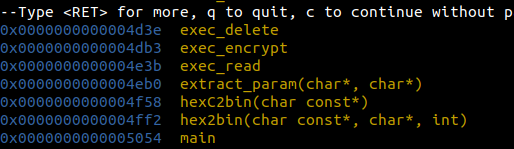
\includegraphics[width=0.7\columnwidth]{Figures/Fig_36.png}
\caption{Partial results of: \textbf{info functions} within GDB.}
\label{fig:gantt}
\end{figure}

To disassemble the \textbf{exec\_encrypt} function the following command within GDB was issued:
\begin{lstlisting}[language=bash, frame=none]
$ disas /r exec_encrypt
\end{lstlisting}

Figure 7.10 depicts the partial output of the above GDB command. It is seen consisting of a range of assembly instructions followed by their corresponding hex values.
\begin{figure}[H]
\centering
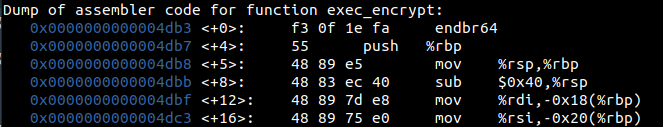
\includegraphics[width=1\columnwidth]{Figures/Fig_37.png}
\caption{Partial results of: \textbf{disas /r exec\_encrypt} within GDB.}
\label{fig:gantt}
\end{figure}

The source code for the injector client also contains a function \textbf{hk\_exec\_encrypt} which represents the detour function to call instead of the original. This function intercepts the plain-text password passed from the browser extension through standard input/output and writes it to a file \textbf{leak.txt} within the users home directory. Due to ASLR (address space layout randomization) within the Linux kernel the location of the \textbf{exec\_encrypt} function changes on each execution cycle. Therefore a means of obtaining the runtime address of the function is required and this is achieved through a call to \textbf{dlsym} within \textbf{initialize}.

In order to jump to the address of the detour function \textbf{hk\_exec\_encrypt} a series of assembly opcodes need to be written to the first few bytes of the detour function. For 64-bit architectures this involves writing the address to jump to into the RAX register and then jumping to the value stored within RAX.

As can be seen in Figure 7.11 the first \textbf{mov} instruction has the following opcode byte sequence: \textbf{0x48, 0xb8} this is then followed the an eight byte address which is stored in little-endian order. Finally the jump to rax is encoded with: \textbf{0xff, 0xe0}. These instruction encodings can be found within the \textbf{jmp\_hook} function of the injector client. When writing these instruction opcodes to memory it is important to set the memory page permissions to writable in order to avoid a segmentation fault. This is accomplished through a call to \textbf{mprotect} within \textbf{jmp\_hook} which sets the memory page permissions. 

\begin{figure}[H]
\centering
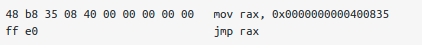
\includegraphics[width=0.8\columnwidth]{Figures/Fig_38.png}
\caption{Assembly jump encoding on x86\_64. RAX method.}
\label{fig:gantt}
\end{figure}

\subsubsection{Method}

The procedure for the experiment first involved compiling the supplied shared library injector \cite{injector} with the following command:
\begin{lstlisting}[language=bash, frame=none]
$ make
\end{lstlisting}

The corresponding output file stored within: \textbf{injector-root/cmd/injector} was then transferred to the root directory of the injector client. Next an instance of google chrome was started (which subsequently started the native host). The injector client was then injected into the native host using the shared library injector with the following command:

\begin{lstlisting}[language=bash, frame=none]
$ sudo ./injector -n "nativehost" client.so
\end{lstlisting}

The user would then proceed to a random login portal, enter a username (test\_user) and password (test\_password) and click the 'Store Credential' button of the browser extension. Finally the file \textbf{leak.txt} would be inspected within the home directory for the leaked password.

Optionally GDB could be attached to the native host to reinspect the \textbf{exec\_encrypt} function with the modified instruction bytes:

\begin{lstlisting}[language=bash, frame=none]
$ gdb -p PID
\end{lstlisting}

\subsubsection{Results}

Figure 7.12 shows the results of the injection of \textbf{client.so} into the native host (\textbf{pingpong} here during testing but named \textbf{nativehost} subsequently). As can be seen the results of injection are successful and the executable code of the injector client is copied over to the native host and the entry point \textbf{initialize} is executed, patching the function \textbf{exec\_encrypt} within the native host.
\begin{figure}[H]
\centering
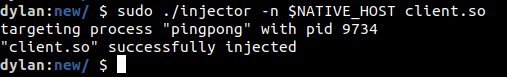
\includegraphics[width=0.8\columnwidth]{Figures/Fig_39.png}
\caption{Result of injection.}
\label{fig:gantt}
\end{figure}

GDB was attached to the native host and the function \textbf{exec\_encrypt} disassembled again to reveal the modified instruction opcodes (Figure 7.13):

\begin{figure}[H]
\centering
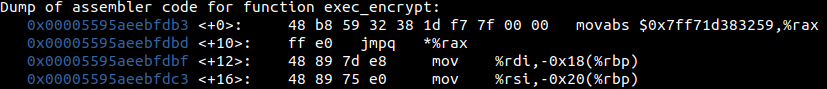
\includegraphics[width=1\columnwidth]{Figures/Fig_41.png}
\caption{Disassembly of \textbf{exec\_encrypt} following injection}
\label{fig:gantt}
\end{figure}

As can be seen in Figure 7.13 the resulting instructions at the detour function have been modified to load the 64-bit address of the detour function \textbf{hk\_exec\_encrypt} into RAX and to then jump to the address stored in RAX. When the original \textbf{exec\_encrypt} function was called, the plain-text password would then be stored in a file \textbf{leak.txt} instead of sending the data over the serial channel to the USB driver MCU.

The contents of \textbf{leak.txt} were then outputted using the command \textbf{cat} (Figure 7.14):

\begin{figure}[H]
\centering
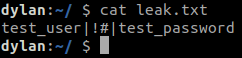
\includegraphics[width=0.45\columnwidth]{Figures/Fig_85.png}
\caption{Output of file \textbf{leak.txt} following injection}
\label{fig:gantt}
\end{figure}

The output is seen to match the credentials entered when the 'Store Credential' button within the browser extension was clicked. The results of this experiment indicate that the native host is susceptible to code injection attacks. Specifically an attacker could craft a malicious shared library object and then inject it into the native host to intercept passwords. However injection requires \textbf{sudo} level privileges which an attacker might not have on a compromised system. 

A countermeasure to code injection might involve scanning the list of shared libraries loaded into an ELF executable and then flagging certain unauthorized shared library objects. Additionally injection relies on an internal call to the Linux specific function \textbf{dlopen}, this function could be detoured itself to fail when trying to load a shared library with a name not on a white-list for example.

\subsection{Attack Surface}

When considering the attack surface of the overall system the degree of isolation between the various software subsystems is important as a vulnerability in one software component may couple to another closely related component. 

Currently encryption is handled on the auxiliary MCU and decryption handled on the software client. The data that is sent over the serial connection (from the nativehost to the auxiliary MCU) during encryption is the plain-text password as well as key modulus. Interception of serial data as highlighted in experiment 1 could lead to credential compromise. However this requires physical access to the serial connection during encryption which is unlikely.

Two authentication steps are required when using the browser extension. The first authentication step consists of a password prompt when the google chrome browser is opened for the first time. This password is stored within local storage in plain-text on the browser and is therefore trivial to bypass for a determined attacker. However the goal of this password authentication step is simply to add a primitive security barrier so that a casual user cannot simply log into accounts on an unattended computer for example. 

The second authentication step requires the presence of an RSA PEM formatted private key in the users home directory (\textbf{key.pem}). If this key file is not present then a new PEM key is generated. This key file is critical and is used to decrypt credentials within the native host (which are passed to the browser extension). This file is unique for each user and a user without a proper key will not be able to decrypt user credentials. This file is designed to be isolated from the browser extension as an alternative would involve RSA private key data in local storage which is not considered secure.

Experiment 1 however also highlighted that the browser extension is vulnerable to malicious modification. It was seen that by embedding a special WebSocket client within the browser extension that a plain-text credential could be compromised. Various other forms of malware, as highlighted in the literature review, could also have been used to compromise the end system including RATs (remote access trojans) which would give an attacker full access to the hosts computing system (which would allow for the interception of \textbf{key.pem}). Malware is therefore a probable attack vector but requires some form of privilege escalation to infect a host and, depending on the user, may be difficult to obtain. 

Phishing is another general technique that may be used by an attacker to gain access to login credentials and requires the crafting of a login page that appears legitimate, often redirecting a user to an attacker controlled server. This is however a more general attack which is not specific to portable (USB-based) password managers.

Currently if an attacker were to acquire access to the USB end system they would be able to dump the contents of the EEPROM and extract file data. However the file data is stored in an encrypted form without any key information. Therefore an attacker would have to bruteforce the RSA primes p and q. For a 1024 bit modulus the bit length of each prime is approximately 512 bits. According to the prime number theorem \cite{wiki_prime} the number of primes smaller than x, n(x), is approximately equal to:

\[ n(x) = \dfrac{x}{\ln x}\]

The number of possible 512 bit primes is therefore given by:

\[\dfrac{2^{513}}{\ln 2^{513}}-\dfrac{2^{512}}{\ln 2^{512}}\simeq 2.8\times 10^{151}\]

The total number of prime pairs then becomes:

\[\dfrac{\left( 2.8\times 10^{151}\right) ^{2}}{2}-2.8\times 10^{151}\simeq 3.9\times 10^{302}\]

As can be seen the number of possible prime pairs is significant which makes brute forcing incredibly difficult for an attacker. The data being encrypted is also padded with PKCS\#1 which means that simple data entropy based attacks become infeasible for larger credentials. 

Rather than compromising a credential directly, experiment 2 aimed at denying users the ability to use services offered by the end host. It was determined that similar to experiment 1, DoS based attacks also require some level of privilege in order to execute malicious code that would interfere with the serial communication protocol at each endpoint. A bug was also found in the way in which the auxiliary MCU parses commands in which a variable size command/data burst would lead to memory exhaustion and device lockup. 

Finally experiment 3 investigated another method of credential extraction, namely code injection. This attack assumes that it is possible for an attacker to modify the CPU instructions in memory of the C++ native host client. An attacker could insert a detour to hook a function performing a critical role such as encryption/decryption to capture login credentials or could insert a shellcode payload to connect to a command and control server similar to experiment 1.

In summary due to the isolation between the encryption and decryption functionality there is no straightforward attack vector. Simple JavaScript code injection would not be sufficient to capture sensitive login credentials as google chrome isolates the browser extension from background (tab based) pages. Only a modification and re-installation of the browser extension itself would prove sufficient to capture credentials at the browser level. Zero-day exploits, which are critical exploits that are known privately (i.e out of the public sphere) however can often lead to RCE (remote code execution) within a browser context, effectively granting system level access to an attacker. These are more complex to execute and google chrome receives regular updates/patches to mitigate publicly disclosed zero-days.

Additionally having access to the USB host device is also not an efficient method at compromising credentials as it was demonstrated that brute forcing would require unrealistic computing capacity that is beyond the reach of most individuals, this is due to the separation of credential data and the encryption key.

It should be noted that ensuring system security is a challenge as there is no model for 'perfect security'. As is the case with reverse engineering, a determined attacker will often find creative exploits or vulnerabilities which mitigate security mechanisms put in place by the original author. An author can however put in place commonsense security mechanisms and barriers to increase the costs involved with exploiting the overall system and this was the methodology used in this report.

